%----------------------------------------------------------------------------
\documentclass{article}
%----------------------------------------------------------------------------
\usepackage[a4paper, top=20mm, bottom=20mm, left=20mm, right=20mm]{geometry}
%----------------------------------------------------------------------------
\usepackage{paracol}
\usepackage{graphicx}
\usepackage{hyperref}
\usepackage[dvipsnames]{xcolor}
\usepackage{lipsum}
\usepackage{fancyhdr}
\usepackage[ngerman]{babel}
\usepackage{csquotes}
\usepackage{float}
\bibliographystyle{ieeetr}
%----------------------------------------------------------------------------
\graphicspath{ {./images/} }
%----------------------------------------------------------------------------
% fancyhdr setup
%----------------------------------------------------------------------------
\pagestyle{fancy}	% activate fancy style
\fancyhf{}			% clear fancy settings
% Header
\fancyhead[L]{Meilenstein 2}
\fancyhead[R]{v1.0}
% Footer
\fancyfoot[C]{Seite \thepage}
\fancyfoot[R]{\today}
% lines
\renewcommand{\headrulewidth}{0.4pt}
\renewcommand{\footrulewidth}{0.4pt}
%----------------------------------------------------------------------------
% first page setup
%----------------------------------------------------------------------------
\title{Teamprojekt}
\author{Adaktylos Leonidas Odysseas, Baumgartner Vincent Vitez, Neda Nikkhousarighiyeh, Alexander Grath}
\date{} % empty date
%----------------------------------------------------------------------------
% reference definitions
% to use references: compile with bibtex then with pdflatex
%----------------------------------------------------------------------------

%############################################################################
\begin{document}
%
\maketitle
%
\thispagestyle{empty} % clear page number
%
% sub-title of the document
\begin{center}
\section*{M2 Low-fidelity Prototypen}
\end{center}

% universität wien logo
\begin{figure}
	\centering
	
\includegraphics[scale=.6]{univie}
\end{figure}
%
\newpage
%
\tableofcontents
%
\setcounter{page}{1} % restart page count at 1
%
\newpage
%
% The \inputs can be change to \include if needed
% put your section in the section folder and only change this document by adding another \input{...}
% the sections are <name>_<chapter>.tex files and do NOT include any document structure code
% thre is nothing fancy going on, the content of the files is just pasted here:
%
\section{Idee Alexander}
\lipsum[1-2]
\section{Idee Leonidas}
\lipsum[1-2]
\section{Idee Neda}
\lipsum[1-2]
\section{Idee Vincent}

\subsection{Grundkonzept}

Die Idee des Low-Fidelity-Prototyps \textit{Wien in Zahlen} ist ein personalisierter Open-Data-Feed für die Stadt Wien. Die App soll nicht wie ein klassisches Datenportal funktionieren, in dem viele Datensätze gleichzeitig angezeigt werden. Stattdessen erhalten Nutzer:innen regelmäßig kurze und verständlich aufbereitete Datenbeiträge in Form von Fact Sheets. Dadurch verbindet die App Elemente einer News-App mit den Möglichkeiten eines Open-Data-Portals.

\subsection{Personalisierter Feed}

Zu Beginn der Nutzung wählen die Nutzer:innen Themen aus, die sie besonders interessieren, zum Beispiel Umwelt, Wohnen, Mobilität oder Energie. Auf Basis dieser Auswahl wird ein persönlicher Feed erstellt. In diesem Feed erscheinen kurze Karten mit aktuellen oder interessanten Datenbeiträgen zur Stadt Wien. Jede Karte gibt einen ersten Überblick und führt bei Interesse zu einem ausführlicheren Fact Sheet. So können Nutzer:innen selbst entscheiden, welche Inhalte sie genauer ansehen möchten.

\subsection{Aufbau der Fact Sheets}

Ein Fact Sheet enthält eine kurze Erklärung des Themas, eine einfache Datenvisualisierung, die verwendete Datenquelle, einen Vergleich sowie den Abschnitt \textit{Was bedeutet das?}. Dieser Abschnitt ist besonders wichtig, weil er die zentrale Aussage der Daten in Alltagssprache erklärt. Die Nutzer:innen sollen nicht nur Zahlen sehen, sondern auch verstehen, welche Bedeutung diese Zahlen für Wien und den Alltag in der Stadt haben.

\subsection{Unterstützung beim Verstehen von Visualisierungen}

Ergänzend gibt es bei jeder Visualisierung ein \textit{Grafik verstehen}-Element mit einem Fragezeichen. Wenn dieses angeklickt wird, öffnet sich eine kurze Erklärung zur jeweiligen Grafik, zum Beispiel wie ein Balkendiagramm gelesen wird. Dadurch unterstützt die App auch Menschen, die wenig Erfahrung mit Datenvisualisierungen oder Statistiken haben.

\subsection{Voting und Frageportal}

Zusätzlich enthält \textit{Wien in Zahlen} ein Voting-System. Damit können Nutzer:innen abstimmen, welche Themen oder Datenfragen in Zukunft aufbereitet werden sollen. Ein Frageportal ermöglicht es außerdem, eigene Fragen zur Stadt Wien einzureichen. Dadurch wird die App nicht nur zu einem Informationsangebot, sondern auch zu einem Mitmach-Format.

\subsection{Ziel der Umsetzung}

Die Umsetzung ist sinnvoll, weil sie Open Data niedrigschwellig, personalisiert und alltagsnah vermittelt. Komplexe Daten werden in kleine, verständliche Einheiten übersetzt, wodurch mehr Menschen einen Zugang zu städtischen Informationen erhalten und sich besser mit Entwicklungen in Wien auseinandersetzen können.
%
\section{Prototyp Alexaner}
\lipsum[1-2]
\section{Prototyp Karte}
\begin{figure}[H]
    \centering
    
\includegraphics[width=0.90\textwidth]{prototype_leonidas.png}
    \caption{Prototyp zur "Karten" App}
    \label{fig:Prototype_Leonidas}
\end{figure}

%
Der Prototyp wurde mit Figma und dem Material 3 Design Kit von Google erstellt. Die Karte ist ein Screenshot vom \href{https://stadtplan.wien.gv.at/}{Stadtplan der Stadt Wien}.
\section{Prototyp Neda}
\lipsum[1-2]
\section{Prototyp Vincent}
\lipsum[1-2]
%
\section{Data Feed - Anpassung}
%
\subsection{Primäre Personas}
%
Benjamin, Leah und Ralph nutzen die App sehr aktiv für ihr Hobby, Bildung und Beruf. Einen lockereren und einfachen Ansatz zur Datendarstellung werden sie sicher wertschätzen, aber 
sie wollen vermutlich mehr. Um "Power Usern" ein besseres Erlebnis zu bieten, wird eine Suchfunktion mit Filtern eingebaut. Standardmäßig kann man mit dieser das aktuell gewählte
Thema durchsuchen, es gibt aber auch weitere Optionen wie Filter, Quellen und ob man z.B.: Den Text oder nur den Titel durchsuchen will.
%
\begin{figure}[H]
    \centering
    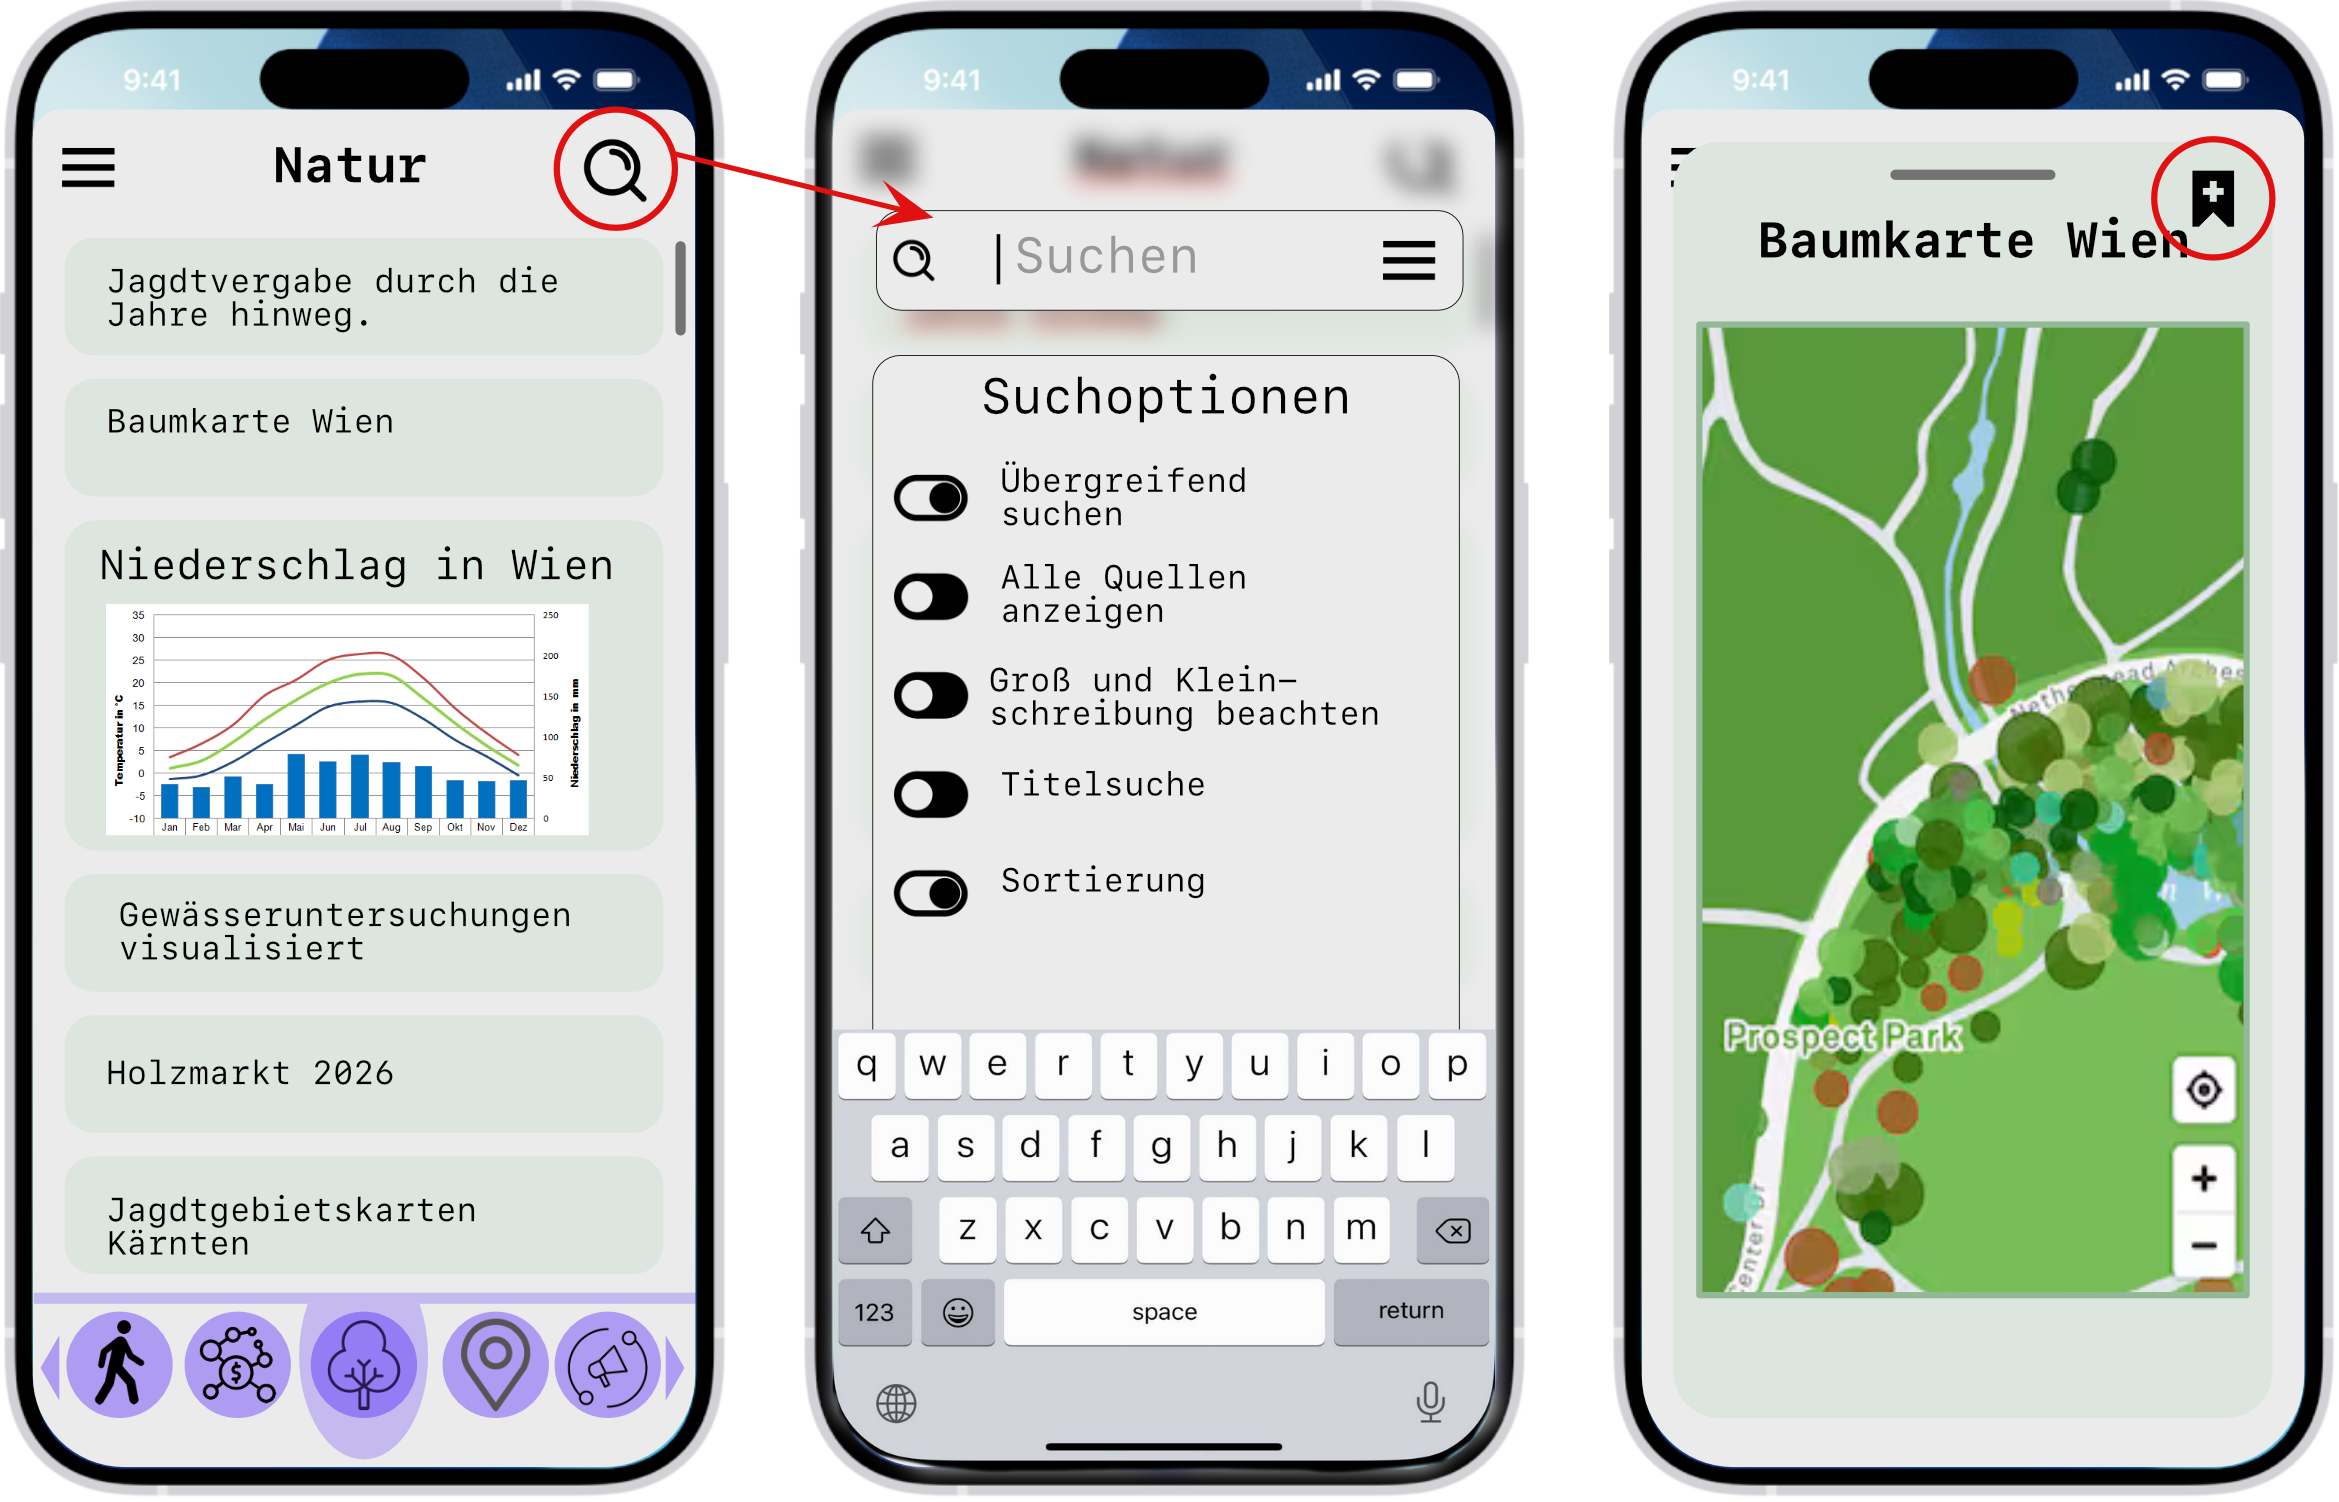
\includegraphics[width=0.90\textwidth]{app_erweiterung_primaer_alexander.png}
    \caption{Erweiterung für Primäre Nutzer}
    \label{fig:Primaere_Erweiterung_Alexander}
\end{figure}
%
\noindent
In die rechte obere Ecke der Hauptseite wird ein Lupensymbol hinzugefügt. Wird dieses angeklickt, dann wird die Suchleiste eingeblendet und der Hintergrund unscharf gemacht.
Die Tastatur öffnet sich automatisch und man kann sofort tippen. Durch Klicken außerhalb der Suchleiste wird die Suche beendet.
Wird das Burgermenü angeklickt, dann öffnen sich die weiteren Einstellungen. Hier können die Suchparameter angepasst werden.
\\
\\
Bei jedem Post wird an die rechte obere Ecke ein "Lesezeichen"-Symbol platziert. Hiermit können die Nutzer den Post für später speichern.
%
\subsection{Sekundäre Personas}
%
Luca, unser Repräsentant der sekundären Personas, ist ein Nutzer, der die App nicht oft nutzt. Während der Nutzung gibt es zwar ein Ziel, aber innerhalb der App bei unseren Daten
wird nichts spezifisch genutzt. Für die sekundären Nutzer werden zwei Dinge hinzugefügt. Erstens wird noch vor der Auswahl der Themen ein weiterer Unterpunkt hinzugefügt: die Daten des Tages/Woche. 
Hier wird den Nutzern ein aktueller und interessanter Post vorgeschlagen. Zusätzlich gibt es noch eine Zufallssuche, hier kann man auf Knopfdruck einen zufälligen Post heraussuchen.
%
\begin{figure}[H]
    \centering
    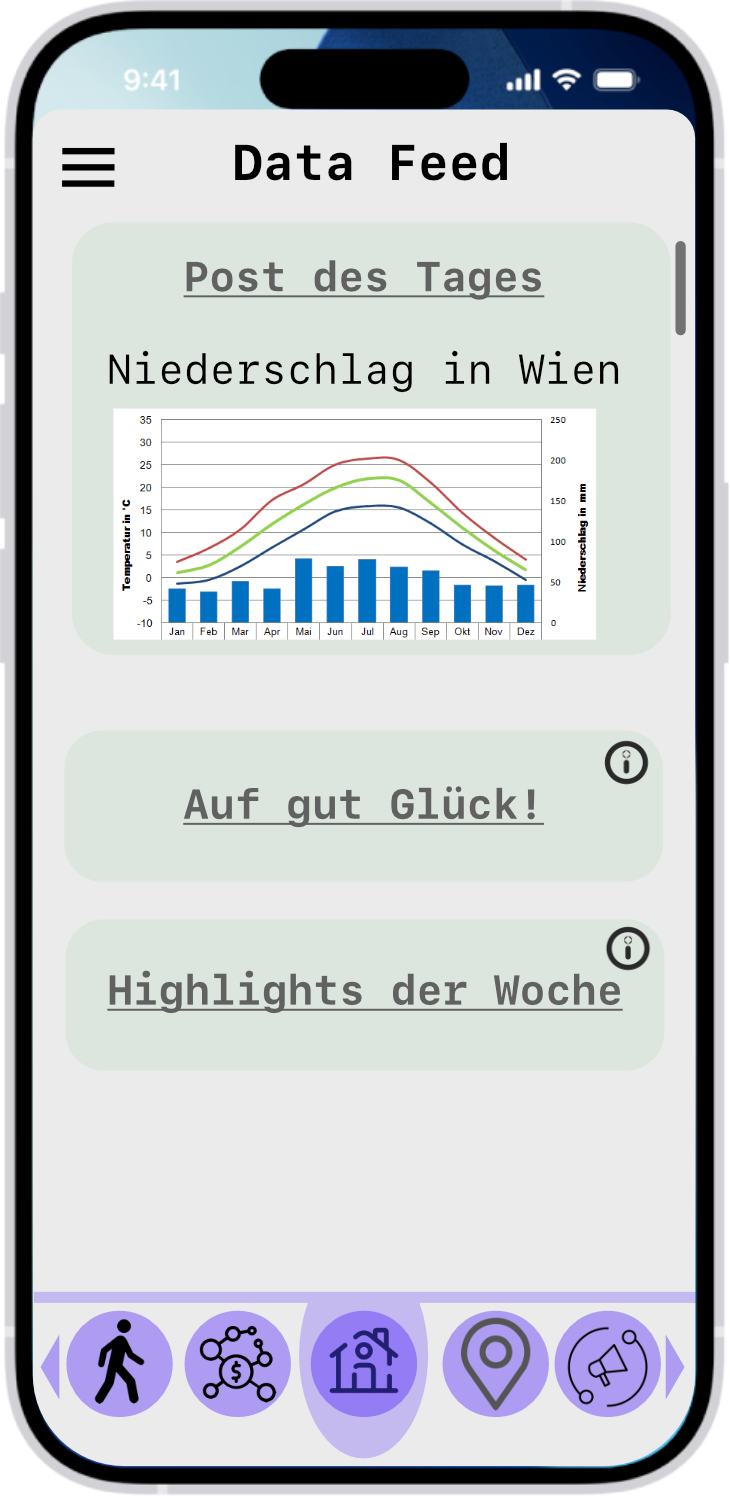
\includegraphics[width=0.30\textwidth]{app_erweiterung_sekundaer_alexander.png}
    \caption{Erweiterung für Sekundäre Nutzer}
    \label{fig:Sekundaere_Erweiterung_Alexander}
\end{figure}
%
\subsection{Negative Persona}
%
Die negative Persona ist jemand, der die dargestellten Daten zweckentfremden will und damit die Meinung anderer manipulieren will. In einer weniger extremen Darstellung
eines negativen Nutzers könnte doch auch jemand versuchen, die Daten entweder falsch auszulegen oder sogar die Daten selber zu verändern.
Innerhalb der App / der UI gibt es hier weniger zu tun. Eher ist es wichtiger, die API und App selbst mit guten Sicherheitsgrundlagen zu programmieren. 
Zusätzlich müssen die rechtlichen Grundlagen gut geklärt sein, wo und wie die Daten weiterverwendet werden dürfen (Lizenzen etc.).
Seitens der Quellen muss es auch klar sein, dass wir keine Verantwortung für die Richtigkeit oder auch den Inhalt der Datensätze übernehmen.
\section{Anpassung Leonidas}
\lipsum[1-2]
\section{Anpassung Neda}
\lipsum[1-2]
\section{Anpassung Vincent}
\lipsum[1-2]
%
\section{Evaluierung Alexander}
\lipsum[1-2]
\section{Evaluierung Leonidas}
\lipsum[1-2]
\section{Story Explorer – Evaluierung}
\lipsum[1-2]
\section{Evaluierung Vincent mit Mitbewohner}

\subsection{Durchf\"uhrung}

\begin{itemize}
    \item Die Testperson war mein Mitbewohner und nicht Teil des Projektteams.
    \item Zu Beginn wurden alle vier Low-Fidelity-Prototypen vorgestellt: \textit{Data Feed}, \textit{Karten-App}, \textit{Story Explorer} und \textit{Wien in Zahlen}.
    \item Zu jedem Prototyp wurden die Grundidee, die wichtigsten Screens und der geplante Nutzungsablauf kurz erkl\"art.
    \item Anschlie{\ss}end wurde die Testperson nach ihrem allgemeinen Eindruck, ihren Pr\"aferenzen und m\"oglichen Verbesserungsw\"unschen gefragt.
    \item Der Fokus lag auf Verst\"andlichkeit, Zugang zu Open Data, hilfreichen Funktionen und unklaren Elementen.
\end{itemize}

\subsection{Ergebnisse}

\begin{itemize}
    \item Positiv wurde bewertet, dass alle vier Prototypen unterschiedliche Zug\"ange zu Open Data anbieten.
    \item Der \textit{Data Feed} wurde als vertraut wahrgenommen, da er an Social-Media-Feeds erinnert.
    \item Die \textit{Karten-App} wurde besonders f\"ur ortsbezogene Informationen als sinnvoll eingesch\"atzt.
    \item Beim \textit{Story Explorer} wurde der gef\"uhrte Ablauf von Thema zu Datensatz zu Story positiv hervorgehoben.
    \item \textit{Wien in Zahlen} wurde positiv bewertet, da Themenauswahl, personalisierter Feed und Fact Sheets einen klaren und alltagsnahen Zugang bieten.
    \item Besonders hilfreich wirkten bei \textit{Wien in Zahlen} das ``Grafik verstehen''-Element und der Abschnitt ``Was bedeutet das?''.
    \item Als bevorzugte Ans\"atze wurden die \textit{Karten-App} f\"ur konkrete Informationen in der Umgebung und \textit{Wien in Zahlen} f\"ur regelm\"a{\ss}iges, einfaches Informieren genannt.
    \item Als Verbesserungsw\"unsche wurden klarere Hinweise zur Aktualit\"at der Daten, sichtbare Quellenangaben und mehr Filterm\"oglichkeiten genannt.
\end{itemize}
%
\section{Arbeitsverteilung}
\lipsum[1-2]
%
\section{KI Nutzung}
%
\noindent
Im Rahmen dieses Meilensteins wurde künstliche Intelligenz unterstützend eingesetzt.
\\
\\
\textbf{Neda Nikkhousarighiyeh:} Die Texte der Abschnitte
\textit{Story Explorer – Idee}, \textit{Story Explorer – Prototyp} und
\textit{Story Explorer – Anpassung} wurden mithilfe eines KI-Sprachmodells
grammatikalisch und sprachlich überarbeitet. Inhalt, Konzept und Ideen
wurden vollständig selbst erarbeitet.

\paragraph{Vincent Baumgartner} 
In den Abschnitten ``Idee'' und ``Prototyp'' wurde K\"unstliche Intelligenz unterst\"utzend zur Textgenerierung sowie zur sprachlichen und grammatikalischen Verbesserung eingesetzt. Die zugrunde liegenden Ideen, Konzepte, Bilder und Prototypen wurden eigenst\"andig erstellt. \url{https://chatgpt.com/share/69e4e631-5a58-8390-a344-443f19b2b895}
%
\newpage
%
% Reference page, can be deleted if not used
%
\bibliography{references}
%
\end{document}